% Instructions to modify this document:
% * Remember to ALWAYS execute "git pull" BEFORE any commit you make!
% * Use the \ToDo{...} command to remark tasks which still need to be done. Add your name in the comment.
% * Use the \input{file.tex} command to split the document into several parts
% * Do not change the current LaTeX coding style to yours. The style and format should be homogeneous along sections.

% To convert .dia diagrams into PDF:
% 1) Create the diagram with dia
% 2) Export it as .eps
% 3) use epstopdf to convert to PDF


\documentclass[a4paper,12pt]{article}

\usepackage[utf8]{inputenc}
\usepackage{amsmath,graphicx}
\usepackage{bm}
\usepackage{amssymb}
\usepackage{algorithm}
\usepackage{algpseudocode}
\usepackage{subfigure}
\usepackage{ifpdf}
\usepackage{url}
\usepackage{color}
\usepackage[hidelinks]{hyperref}
\usepackage{multirow}
\usepackage{datetime}
\usepackage{comment}
\usepackage{float} % To put figures in their exact place with \begin{figure}[H]
\usepackage{longtable}
\usepackage{tabularx}
\usepackage{listings}
\usepackage{xcolor}


\newcolumntype{L}[1]{>{\raggedright\arraybackslash}p{#1}}
\newcolumntype{C}[1]{>{\centering\arraybackslash}p{#1}}
\newcolumntype{R}[1]{>{\raggedleft\arraybackslash}p{#1}}


% Definitions and commands
\def \np{\vskip 0.25 cm}
\def \ap{\vskip 0.15 cm}

% JSON listing (see 
%  http://tex.stackexchange.com/questions/83085/how-to-improve-listings-display 
% -of- json-files)
\colorlet{punct}{red!60!black}
\definecolor{background}{HTML}{EEEEEE}
\definecolor{delim}{RGB}{20,105,176}
\colorlet{numb}{magenta!60!black}

\lstdefinelanguage{json}{
    basicstyle=\footnotesize\ttfamily,
    numbers=left,
    numberstyle=\scriptsize,
    stepnumber=1,
    numbersep=8pt,
    showstringspaces=false,
    breaklines=true,
    frame=lines,
    backgroundcolor=\color{background},
    literate=
     *{0}{{{\color{numb}0}}}{1}
      {1}{{{\color{numb}1}}}{1}
      {2}{{{\color{numb}2}}}{1}
      {3}{{{\color{numb}3}}}{1}
      {4}{{{\color{numb}4}}}{1}
      {5}{{{\color{numb}5}}}{1}
      {6}{{{\color{numb}6}}}{1}
      {7}{{{\color{numb}7}}}{1}
      {8}{{{\color{numb}8}}}{1}
      {9}{{{\color{numb}9}}}{1}
      {:}{{{\color{punct}{:}}}}{1}
      {,}{{{\color{punct}{,}}}}{1}
      {\{}{{{\color{delim}{\{}}}}{1}
      {\}}{{{\color{delim}{\}}}}}{1}
      {[}{{{\color{delim}{[}}}}{1}
      {]}{{{\color{delim}{]}}}}{1},
}

\lstset{language=Bash, basicstyle=\color{gray}}

\newcommand{\ToDo}[1]{\textcolor{magenta}{\textbf{[ToDo]} \textbf{#1}}}
\newcommand{\miguel}[1]{\textcolor{magenta}{\textbf{[Miguel]} \textbf{#1}}}


\begin{document}


\begin{titlepage}

\begin{center}
\vspace*{-1in}

\vspace*{0.6in}
\begin{Large}
\textbf{The IPOL Demo System 2.0 \\Technical documentation} \\
\end{Large}

\vspace*{0.6in}

\small{Compiled on \today\ at \currenttime}

\vspace*{0.6in}
\rule{80mm}{0.1mm}\\
\vspace*{0.1in}
\end{center}

\end{titlepage}

This document contains technical documentation for the IPOL Demo System 2.0. Specifically, the architecture of the service-oriented platform, its modules, and the real-time template generation of demos from their textual description.
\vspace*{0.6in}

\textbf{Software engineers and external consultats, past and present (in alphabetical order):}


Martín Arévalo

José Arrecio

Miguel Colom

Carlos Escobar

Vincent Firmin

Karl Krissian

José Luis Lisani

Alexis Mongin

Nelson Monzón

\vspace*{0.2in}

\textbf{Project direction and team coordination}

Miguel Colom - \url{http://mcolom.info}



%\maketitle
\newpage

\tableofcontents
\newpage
\listoffigures
\newpage

% Introduction
\section{Introduction}
\ToDo{Incomplete section!}

The system is built as a service-oriented architecture \cite{neuman2015building}.
The functionality is decomposed into a set of independent, self-contained microservice modules which communicate with each other via an API.

By splitting the monolithic application into smaller modules and decoupling interdependencies (between apps, dev teams, technologies, environments, and tooling), the system gains in terms of scalability, parallel development, easier debugging, and complexity isolation.

\begin{figure}[!ht]
\centering
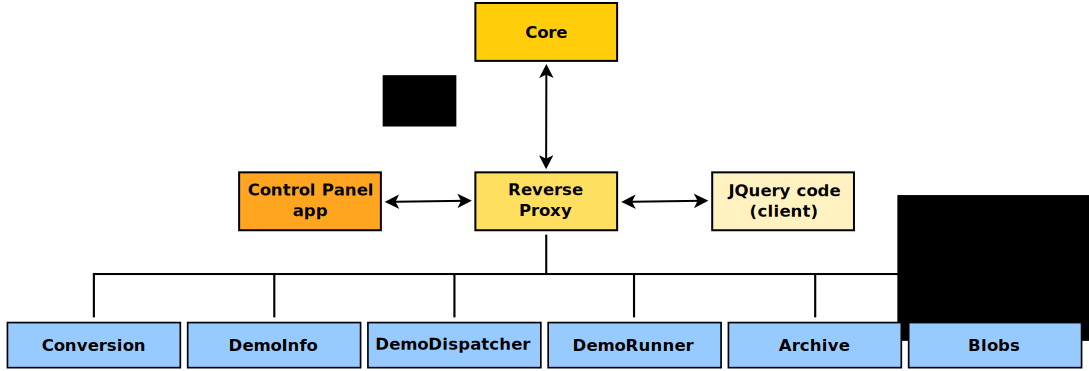
\includegraphics[width=0.8\linewidth]{architecture/images/architecture.pdf}
\caption{Modular system architecture.} 
\label{fig:architecture}
\end{figure}


% Project management and development methodology
% Project management and development methodology

\section{Development Methodology and Project Management}
The current IPOL project tries to follow the best practices in software engineering. Specifically, for this kind of project we found that Continuous Integration was a good choice in order to achieve fast delivery of results and ensuring quality. Continuous Integration is a methodology for software development proposed by Martin Fowler~\cite{fowler2006continuous} which consists on making automatic integrations of each increment achieved in a project as often as possible in order to detect failures as soon as possible. This integration includes the compilation and software testing of the entire project.

It is a set of policies that, together with continuous deployment, ensures that the code can be put to work quickly. It involves automatic testing in both integration and production environments. In this sense, each contribution in the IPOL system is quickly submitted and several automatic test are performed. If any of these tests fail the system sends an email indicating the causes.
%
Another advice of Continuous Integration is minimal branching. We use two. On one hand, master is the default branch and where all the contributions are committed. It is used for the development, testing and this continuous integration; on the other hand, the prod branch is used only in the production servers. It is merged with master regularly.
%
We use two different environments: integration and production. The integration server is where the master branch is pulled after each commit. The prod branch is used for the production servers and the code in this branch is assumed to be stable. However, the code in the integration server is also assumed to be stable and theoretically the code in the master branch could be promoted to production at any time once it has been deployed to the integration server and checked that is is fully functional and without errors. 

Quality is perhaps the most important requirement in the software guidelines of the IPOL development team. The code of the modules must be readable and the use of reusable solution is advised~\cite{GoF}. The modules must be simple, well tested and documented, with loose interface coupling, and with proper error logging. Note that it is not possible to ensure that any part of the IPOL will not fail, but in case of a failure we need to limit the propagation of the problem through the system and to end up with diagnostic information which allows to determine the causes afterwards.
%
Refactoring~\cite{fowler1999refactoring} is performed regularly and documentation is as important as the source code. In fact, any discrepancy between the source code and the documentation is considered as a bug.

Another tool used by the team is Trello. It allows to track the tasks of the project accoding to their current state (not assigned, assigned but not stated, assigned and in development, and finished). When a task arrives to the ``Finished" step, it is reviewed by the Project Director and archived (task totally finished) or moved back to development if more work is needed.

\begin{comment}
[ToDo]: move this to Sysadmin doc
The {\tt prod} branch was created with:
\begin{verbatim}
git checkout -b prod
git push --set-upstream origin prod
\end{verbatim}

The .git/config ends up as:

\begin{verbatim}
[core]
	repositoryformatversion = 0
	filemode = true
	bare = false
	logallrefupdates = true
[remote "origin"]
	url = git@github.com:mcolom/ipolDevel.git
	fetch = +refs/heads/*:refs/remotes/origin/*
[branch "master"]
	remote = origin
	merge = refs/heads/master
[branch "prod"]
	remote = origin
	merge = refs/heads/prod
\end{verbatim}

To merge {\tt prod} with {\tt master:}
\begin{verbatim}
git checkout prod
git merge master
git push
git checkout master
\end{verbatim}
\end{comment}


% The Core module
\section{The Core module}
The Core is the centralized controller of the whole IPOL demo system. It controls the execution of the experiments and delegates tasks such as data pre-processing (Conversion module), execution dispatching (Dispatcher module), algorithm execution (DemoRunner module), archiving experiments (Archive module), or retrieving demo metadata, among others. It also sends email notifications when failures are detected during the execution of a demo, bad constructed DDLs or any other problem that needs to be notified to the user, the technical staff, or the IPOL editors.

When an execution is requested, it first obtains its textual description (its DDL) from the DemoInfo module. Then, it asks for the workload of the different DemoRunners and gives this information to the Dispatcher module in order to pick the best DemoRunner according to the Dispatcher's policy. The next step is to ensure that the source codes are compiled and updated in the corresponding DemoRunner. If the demo uses a DemoExtras file it is updated with its last version.

For the execution, the Core creates a run folder, copies the input data, and delegates any eventual pre-processing to the Conversion module. The run folder is identified by an unique key and it is created inside a folder which can be accessed by any machine of the IPOL's architecture. Therefore, all the DemoRunner machines can access the shared folder where the executions are performed. The DemoExtras are common files that are also visible and centralized.

Once the execution folder is ready, the corresponding DemoRunner runs the algorithm with the parameters and inputs set by the user. The Core waits until the execution has finished or after a timeout. Finally, the Core asks the system to store the experiment if the input data came from original data (uploaded by the user without private mode) or if the DDL specified to save all the executed experiments.

In case of any fatal failure (say, a conversion if needed but forbidden in the DDL, or the program of the article crashed), the Core terminates the execution and stores the errors in its log file. Eventually, it will send warning emails to the technical staff of IPOL (internal error) or to the demo editors.

Note that the Core does not need to know to which module it needs to delegate any operations, but instead simply requests the services using the IPOL API (see Sec. \ref{sec:reverse_proxy})

\subsection{DemoExtras}
\label{sec:demoextras} 
For the execution of some demos it is necessary some support code or data, which we refer to as \emph{DemoExtras}. This is not part of the peer-reviewed or published material, and it is only used by the demo.

The support files are stored in a package (say, .tar.gz, .zip, .tar, ...) in the DemoInfo module. Also, a copy of this compressed file is stored in the ``dl\_extras'' folder in the ``shared\_folder'' for comparison reasons. \ToDo{This mechanism should be explained in the demoInfo module section of the doc.}

The first time a demo is executed, the demos extras are decompressed in the ``DemoExtras'' folder in the ``shared\_folder''. At each execution the Core checks the date and the size of the compressed file in the ``shared\_folder'' with the one stored in demoInfo. \ToDo{This mechanism should be explained in the demoInfo module section of the doc. A diagram would be useful.}

The possible results from the check are:
\begin{itemize}
    \item \textbf{Date and size match}: nothing is done
    \item \textbf{Date or size do not match}: the DemoExtras are downloaded again
    \item \textbf{DemoExtras deleted in demoInfo}: all DemoExtras files related to that demo are deleted in the ``shared\_folder''
\end{itemize}

\subsubsection{Serving static content}
The {\tt html} directory of the demoExtras is served staticly by the system to allow the web interface access this data. It can be useful to show extra graphics or videos, or to allow the download of datasets in some especial demos.

For example, if in the demoExtras package of demo \#125 it exists a file ``image.png", it will be served from \url{http://ipolcore.ipol.im/demo/clientApp/static/125/image.png}


\subsection{Editor-controlled demo failures}
The Editor has the possibility to detect that some conditions are not met and notify the system that the execution of the demo failed, even if the program did not crash or the running script exited with a sucessful exit code. Indeed, a demoExtras script in the demo could check, for example, if the aspect ratio of the image is what the algorithm excepts, and prevent the actual execution.

The mechanism is simple: the editors can write a "demo\_failure.txt" file and stop the execution with an exit
code 0. The Core interprets the presence of this file as the demo itself signalling a problem.

For example, this code is used in one of the demos:
\paragraph{Example}:\\
\begin{verbatim}
imageSize=$(identify -format '%w+%h' input_0.png)
maskSize=$(identify -format '%w+%h' mask.png)

if [ $imageSize != $maskSize ]
then
  echo "Input error: input and mask have different sizes." >> demo_failure.txt
  exit 0
fi
\end{verbatim} 


\subsection{Interactive controls}
These are available in order to let the user draw on top of blobs. When adding an interactive control to the inputs of a demo, the core module will create files according to the data the interface sends before actual execution of the demo code. Here's a brief explanation for each kind of control.

\subsubsection{Mask control}
 For each input the core module will save an image with the name mask\_n.png, where 'n' is the number of the input with said control. This image comes from the client-side inside the run request.

\subsubsection{Dots and lines control}
The resulting text file will contain one line per coordinate on the image in a file in the execution folder, it will be named inpainting\_data\_n.txt where 'n' is the number of the input with said control.

Lines control will have the same result and processing by the core module as the dots control.

% The Proxy module
% Nginx as a reverse proxy

\section{Nginx as a reverse proxy}
\label{sec:reverse_proxy}
The IPOL project uses Nginx as a reverse proxy in order to redirect internet requests to the servers in the 
internal network. When Nginx receives a request, it decides which module it hast to send and so which machine that module is, 
then fetches the response, and sends it back to the client. With Nginx we implement private demos, microservise architecture 
patter and serve static files used by the clients.

\subsection{Static files}
The control panel as a Django web application needs to be compiled everytime the files change, so in order to serve the 
application Django offers a cli tool to collect all static files. Nginx serves all the static files used by the application and exposes them 
under a public route.

\subsection{API routing}
Nginx is also used to redirect incoming requests to the corresponding port and direction inside the machine where the module is 
running. Each modules has an internal file (sites-available) that decides where to route the request and deliver it to the desired endpoint.

\subsection{Private demos}
The IPOL system provides private demos that requires authentication by username and password. The ID of these demos begin with 
33333001. In this sense, Nginx can detect when a private demo is requested and it can forbid the access if the authentication fails.

% The Blobs module
\section{The Blobs module}

\subsection{Introduction}
\label{sec:blobs_introduction}
The Blobs module introduction


% The Archive module
\section{The Archive module}

\subsection{Introduction}
\label{sec:archive_introduction}

%\paragraph{Introduction} \hspace{0pt} \\
The archive module is a standalone application destined to communicate with other modules using webservices. It is designed to implement a stable, simple and scalable system for archiving all experiments done with IPOL.

\paragraph{Technologies used} \hspace{0pt} \\
The archive module, written in Python, is using the cherrypy framework for webservices, the mako template library for webpage rendering, Python Image Library for thumbnails creations, and the python-magic library available on pip (not to be mistaken with python-magic5 which is the one available on ubuntu's default APT repositories). The module communicates using JSON, both in input and output. The database engine used is SQLite.

\subsection{Architecture}

\paragraph{Module composition} \hspace{0pt} \\
The module is composed of very few files, the code itself in ``module.py'', a cherrypy configuration file ``archive.conf'', two mako HTML templates, and a database. It will also need 4 directories, respectively for storing blobs, thumbnails, the database and logs.

\paragraph{Module architecture} \hspace{0pt} \\
The module is composed of a class, 'Archive', encapsulating the data needed to function. The services offered by the module are all methods of this class. The cherrypy framework provide the abstraction for making the methods available as webservices. \\
Upon starting the module, the cherrypy engine is launched, an object of the Archive class is created, and the cherrypy configuration is loaded from ``archive.conf''. If they don't exist, both the database and the directories needed for the storage of blobs, logs, the database and thumbnails will be created, provided that the user launching the module has the necessary rights. Otherwise, the module will not start. These directories are indicated in the cherrypy configuration for maximum configurability, if they are missing from it, the module will not start. \\
The webservices communicate with the server via arguments given through URL, as unicode strings directly passed to the methods. \\
The services all connect to the database in a thread-safe way, instanciating its own connection when called, commiting when done if there are modifications, or rollbacking, if there is an error, and closing the connection. \\
There is a logger initialised with the Archive object, writing errors in ``error.log'' in the logs directory given in the configuration file.

\subsection{Database design}

The database contains 3 tables : experiments, blobs, and correspondence.\\
Each experiments, and each blobs are defined individually, and linked to each-others in the correspondence table, assuring a many-to-many connection. It is worth noting that the database does not save duplicates of the same blob. \\

\ToDo{[Miguel] The right name for the ``correspondence" table is \emph{Junction table}. You can keep the name ``correspondence", but explain in the text that it is a junction table.}

\begin{tabular}{|l|c|r|}
  \hline
  experiments & blobs & correspondence \\
  \hline
  id & id & id \\
  id\_demo & hash & id\_experiment \\
  params & type & id\_blob \\
  timestamp & format & name \\
  \hline
\end{tabular} \\

\paragraph{Experiments table} \hspace{0pt} \\
The experiments table is defined as such : the id field, that stores the unique id of the experiment ; the id\_demo field, that stores the id of the IPOL demo used for the experiment ; the params field, which is a JSON string whose format varies from demo to demo ; and finally the timestamp field.

\paragraph{Blobs table} \hspace{0pt} \\
The blobs table is defined as such : the id field, that stores the unique id of the blob ; the hash field, that stores the hash of the blob computed with sha1, the type field, that stores the extension of the blob (e.g. ``jpeg'' or ``png''), and the format field, that stores the media format of the blob : it is a string, either ``audio'', ``video'' or ``image''. \\
The physical location of a blob is ``blob\_dir as defined in the configuration file'' + ``hash of the blob'' + ``.'' + ``type of the blob''.

\paragraph{Correspondence table} \hspace{0pt} \\
\ToDo{[Miguel] You can keep the name ``correspondence", but explain in the text that it is a junction table.}
The correspondence table is defined as such : the id field ; the id of the experiment and the id of the blob that is linked to said experiment, and the name field, which indicates the role of the blob in the experiment (example : ``input'' or ``denoised''). A foreign key constraint allowing cascade delete is put on the field id\_experiment, referencing the id of an entry in the experiment table, for automatic data deletion.

\subsection{Services}

\paragraph{Adding an experiment to the archive} \hspace{0pt} \\
Example :
\begin{verbatim}
http://<localhost>:<port>/add_exp_test?demo_id=42&blobs=
<json_blobs>&parameters=<json_parameters>
\end{verbatim}
The method ``add\_experiment'' takes in the entry of the id of the demo used ; a JSON string of the format : 

\begin{verbatim}
{
    url_blob : name,
    ...
}
\end{verbatim}

containing a description of each blob used by and produced by the experiment, with their temporary URLs and names ; and a JSON string describing the parameters of the demo used for the experiment. It will add an experiment to the database by creating a new entry in the experiment table. If the blobs used by and produced by the experiment aren't already in the database, it will copy them in the directory given in the configuration file, and create a thumbnail for the images. It will return a json string containing the status of the operation, OK if it succeeded, KO if there was an error and the operation wasn't performed, as such :

\begin{verbatim}
{
    status : OK/KO
}
\end{verbatim}

If status is KO, a log describing the error will be written.

\paragraph{Deleting an experiment from the archive} \hspace{0pt} \\
When removing an experiment from the database via the method ``delete\_experiment'', every blob linked to this experiment and only to this experiment is removed. After that, all the entries in the correspondence table referencing this experiment are removed automatically due to a foreign key constraint. It return a json response containing the status of the operation of the same format as the return of the method ``add\_experiment''. The method shouldn't be called anywhere else than through the user interface described later.

\paragraph{Deleting a blob from the archive} \hspace{0pt} \\
Due to a many-to-many link between blobs and experiments in the database, a blob has a lot of dependencies : it has of course the experiments using this blobs, but also the blobs linked to these experiments. For deletion of a blob from the archive, the precedent service is called on each experiment the blob is part of, assuring that no orphan data stay in the database (e.g. experiments linked to removed blobs or blobs linked to removed experiments). The method implementing this service is ``delete\_blob\_w\_deps''. It return a json response containing the status of the operation in the same format as the return of the method ``add\_experiment''. The method shouldn't be called anywhere else than through the user interface described later.

\paragraph{Getting data \ToDo{[Miguel] use a more specific word than ``data"} from an archive page} \hspace{0pt} \\
Example :
\begin{verbatim}
http://<localhost>:<port>/page?demo_id=42&page=3
\end{verbatim}
The method ``page'' returns a JSON response with, for a given page of a given demo, all the data of the experiments that should be displayed on this page. Twelve experiments are displayed by page. For rendering the archive page in the browser, the JSON response should be parsed and interpreted in a dedicated template furnished by the front-end of another module. The JSON response is formatted this way : 
\begin{verbatim}
{
    status :  OK/KO,
    experiments : [
        {
            date : timestamp_example, 
            files : [
                {
                    url : url_example,
                    id : id_example,
                    name : name_example,
                    url_thumb : url_thumbnail_example
                }
            ... ],
            id : id_example,
            parameters = {parameters_example...}
    ... ],
    id_demo : id_demo_example,
    nb_pages : nb_pages_example
}
\end{verbatim} 

\paragraph{Administrator interface for removing blobs/experiments} \hspace{0pt} \\
Example :
\begin{verbatim}
http://<localhost>:<port>/archive_admin?demo_id=42&page=3
\end{verbatim}
The only user interface furnished by the archive module is for removing blobs or experiment in a convenient manner. It uses the json response of the precedent service and renders the ``archive\_admin\_tmp.html'' template displaying a page of archives for given demo, allowing the deletion of both blobs and experiments by simply linking to two other services calling deletion methods and updating the template. In case of error, for example when invalid data is given through URL, ``error.html'' is rendered.

\paragraph{Shutdown} \hspace{0pt} \\
Example :
\begin{verbatim}
http://<localhost>:<port>/shutdown
\end{verbatim}
The method ``Shutdown'' shuts down the archive application when called. It returns a json response containing the status of the operation.

\paragraph{Other services} \hspace{0pt} \\
Other services features the method ``ping'', simply for checking if the module is up, and the method ``stats'', formatted this way :
\begin{verbatim}
{
    status : OK/KO,
    nb_experiments : x,
    nb_blobs : y
}
\end{verbatim}
Example :
\begin{verbatim}
http://<localhost>:<port>/ping
\end{verbatim}
Example :
\begin{verbatim}
http://<localhost>:<port>/stats
\end{verbatim}


% The Demo Info module
\section{DemoInfo module}
This module store the textual description of the demo and allows to ask for specific sections of it. It also stores other demo-related information, as:
\begin{itemize}
\item Demo id
\item Abstract
\item Title 
\item Authors list
\item Authors email list
\item Article URL
\item State (inactive,preprint, published)
\item Demo editor
\item Demo editor email
\item Demo zip file containing demo DDL 
\item Demo DDL JSON
\end{itemize}

This module will be used by the control panel module, the demo will be extracted from the zip file, it will be created in Demoinfo module, The blobs will be added to Blobs module.

\subsection{ demoinfo module structure}
This Module is formed by:
\begin{itemize}
\item model.py where the db structure, the DAO (Data access object) classes and some helper classes (Demo, Author and Editor) are defined. It provides a layer of abstraction over the DB.
\item demoinfo.conf it's the cherrypy config for the webservices module.
\item demoinfo.py it's the webservices module.
\item testdemoinfo.py it's the tests to check that the webservices work.
\item testdemoinfo.conf it's the cherrypy config for testing.
\end{itemize}

\subsection{The model (database) structure}
The model of this module id formed by the following tables:

\begin{figure}[!ht]
\centering
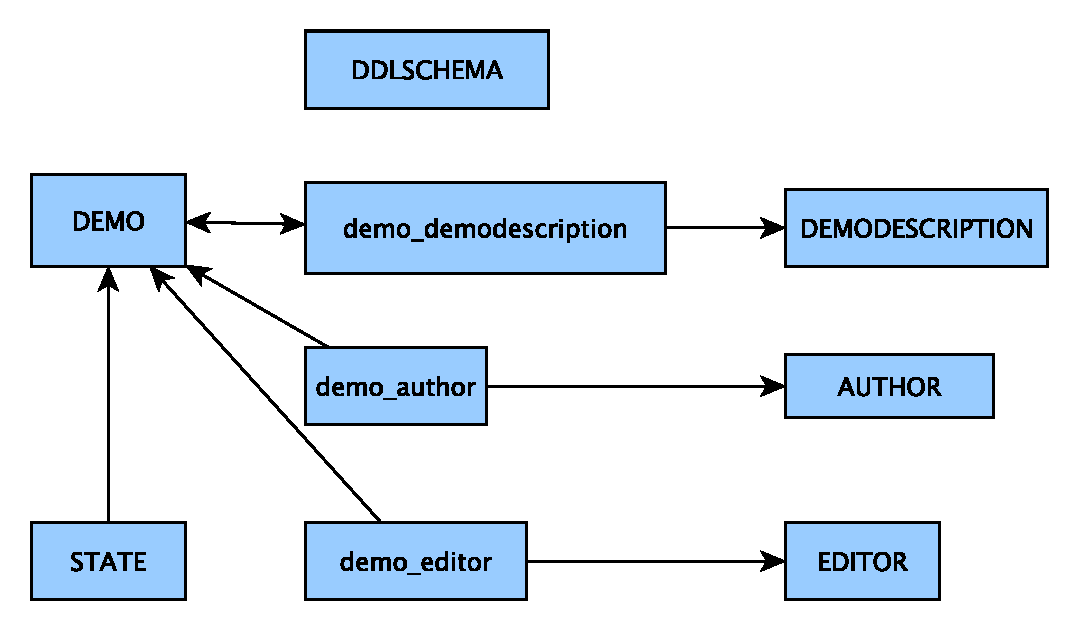
\includegraphics[width=0.8\linewidth]{demo_info/images/demoinfo_model.pdf}
\caption{Demoinfo Database Model.} 
\label{fig:demoinfo_model}
\end{figure}

Note that states is the table for the demo's state (Published,preprint...)
Demodescription table is where the demo description language (DDL) for each demo is stored.
A demo may be created without a DDL (but you will need to provide one so you can run it)
Ddlschema is not used at the moment, but it has been created so that a schema validation can be done to the DDL of each demo, if a user provides a valid json for the DDL but this json is not a valid DDL , whe should be able to detect thisand return an error.

\subsection{Web services available}
This module provides a set of webservices, those that return data can be called with GET or other HTML methods, those that delete,create or update data can be called only by POST.
These webservices are shown grouped by functionality, 


DEMO

\begin{itemize}
\item  demo\_list(self)
\item  demo\_list\_by\_demoeditorid(self,demoeditorid\_list)
\item  demo\_list\_pagination\_and\_filter(self,number\_elements\_page,page,qfilter=None)
\item  demo\_get\_authors\_list(self,demo\_id)
\item  demo\_get\_available\_authors\_list(self,demo\_id)
\item  demo\_get\_editors\_list(self,demo\_id)
\item  demo\_get\_available\_editors\_list(self,demo\_id)
\item  demo\_get\_demodescriptions\_list(self,demo\_id,returnjsons=None)
\item  read\_demo\_metainfo(self, demoid)
\item  read\_demo\_metainfo\_by\_editordemoid(self, editordemoid)
\item  add\_demo(self, editorsdemoid, title, abstract, zipURL, active, stateID, demodescriptionID=None, demodescriptionJson=None)

Allows you to create a demo
- allow only post
- only creating the demo
- creating the demo and assigning an existing ddl (with id demodescriptionID) to it
- create the demo and create a ddl , with the json passed by param (demodescriptionJson)

\item  delete\_demo(self,demo\_id,hard\_delete = False)
allow only post
\item  update\_demo(self,demo)
allow only post
\end{itemize}


AUTHOR

\begin{itemize}
\item  author\_list(self)
\item  author\_list\_pagination\_and\_filter(self,number\_elements\_page,page,qfilter=None)
\item  read\_author(self, authorid)
\item  author\_get\_demos\_list(self,author\_id)
\item  add\_author(self,name, mail)
allow only post
\item  add\_author\_to\_demo(self,demo\_id ,author\_id)
allow only post
\item  remove\_author\_from\_demo(self,demo\_id ,author\_id)
allow only post
\item  remove\_author(self,author\_id)
allow only post
\item  update\_author(self,author)
allow only post
\end{itemize}


EDITOR

\begin{itemize}
\item  editor\_list(self)
\item  editor\_list\_pagination\_and\_filter(self,number\_elements\_page,page,qfilter=None)
\item  editor\_get\_demos\_list(self,editor\_id)
\item  read\_editor(self, editorid)
\item  add\_editor(self,name, mail)
allow only post
\item  add\_editor\_to\_demo(self,demo\_id ,editor\_id)
allow only post
\item  remove\_editor\_from\_demo(self,demo\_id ,editor\_id)
allow only post
\item  remove\_editor(self,editor\_id)
allow only post
\item  update\_editor(self,editor)
allow only post
\end{itemize}

DDL

\begin{itemize}
\item  read\_demo\_description(self, demodescriptionID)
\item  read\_last\_demodescription\_from\_demo(self,demo\_id,returnjsons=None)
\item  add\_demodescription\_to\_demo(self,demo\_id, demodescription\_id)
allow only post
\item  add\_demo\_description(self,demoid=None,inproduction=None)
allow only post
\item  add\_demo\_description\_using\_param(self, demojson,inproduction = None)
\item  update\_demo\_description(self, demodescriptionID)
\end{itemize}

MISCELLANEA

\begin{itemize}
\item  index(self)
\item  ping(self)
\item  shutdown(self)
\item  stats(self)
\item  read\_states(self)
\end{itemize}


\subsection{Module testing}
To test this module enter test folder and run 
\begin{lstlisting}[language=Python,firstnumber=1]
python -m unittest discover.
\end{lstlisting}

To perform manual testing use curl or poster plugging for firefox (remember that some will only work with post requests) but in testdemoinfo.py, in the last tests you will find a working example of how to use some webservices using the request python library.
If you add webservices, please add the corresponding tests.


% The Demo Dispatcher module
\section{DemoDispatcher module}
\label{se:DemoDispatcher}
In order to distribute the load in several machines, this module checks the work load of each known DemoRunner modules and starts an algorithm demo execution on the less loaded machine. The process is done transparently and from the outside this is the only visible module, since the actual DemoRunners are not directly accesible.

It use a FIFO, that is a method of queuing process, for dispatching the different experiments. A machine for the demo runner sne

% \begin{algorithm}[!htbp]
% \caption{Dispatcher}
% \label{al:pyramidal_structure}
% \While{q not empty}
%     \State $ e_{i} \leftarrow q.extract()$
%     \State $ Dr = find\_dr()$
%     \State $ h = get\_id\_e(e_{i})$
%     \State $ notify_dequeue(h) $
%     \State $ Dr\_exec(e_{i}) $
%     \State $ Notify\_execution(h) $ 
% \EndWhile
% \end{algorithm}

\ToDo{Document it!}


% The Demo Runner module

\section{DemoRunner module}
\label{se:DemoRunner}
The DemoRunner module has two main tasks. The first is to inform the DemoDispatcher about the load of the machine where it is running. The second task is to execute an algorithm given the parameters and store the results in a temporary directory. It is a requirement that the temporal results can be accessed by different users using the URL (for example, it may contain a key which identifies a specific experiment).

It can obtain the system load from {\tt /proc/loadavg}. The first three numbers are the load averages for the past 1, 5, and 15 minutes. Load averages are not normalized for the number of CPUs in a system, so a load  average  of 1 means a single CPU system is loaded all the time while on a 4 CPU system it means it was idle 75\% of the time.
\ToDo{Document it!}


% The Control Terminal 
\subsection{The Control Terminal}

The Control Terminal is an standalone application intended for system administration which allows to start, stop, and query the status of each of the IPOL modules. It reads the IPOL configuration from the XML files at {\tt ipolDevel/ipol\_demo/modules/config\_common}.

\subsubsection{Structure}
The Control Terminal is a command-line application to control the IPOL modules at each environment. The terminal is set to particular  enviroment to send the commands to the server in that environment. For example, the local, integration, or production environments. The current environment can be get or set with the {\tt env} command.

\paragraph{XML files} \hspace{0pt} \\
The XML files {\tt modules.xml} and {\tt demorunners.xml} are used by the IPOL modules when started. The Terminal reads these configuration files when started or when the environment is changed.

In {\tt modules.xml} the fields are:
\begin{itemize}
    \item module: the name of the module
    \item server: the host name of the server
    \item serverSSH: the name of the server (used to ssh it)
    \item path: the physical path of the module in the server
    \item command: it declares a command that the module is able to execute
\end{itemize}

The {\tt demorunners.xml} lists and configures each of the demoRunners in that enviroment.

\subsubsection{Commands}
\paragraph{start} \hspace{0pt} \\
Usage: {\tt start <module>}

It starts the specified module by ssh'ing to the server where the module is physically located and invoking the {\tt start.sh} script.
The {\tt ping} command might be executed right after to check if the module is indeed up.

\paragraph{ping} \hspace{0pt} \\
Usage: {\tt ping <module>}

It pings the module to check that it is responsive.

\paragraph{shutdown} \hspace{0pt} \\
Usage: {\tt shutdown <module>}

It shutdowns the specified module.

\paragraph{info} \hspace{0pt} \\
Usage: {\tt info <module>}

It prints the list of available commands for the specified module.

\paragraph{modules} \hspace{0pt} \\
Usage: {\tt modules}

It displays the list of the modules in the IPOL system.

\paragraph{env} \hspace{0pt} \\
Usage: {\tt env <environment>}

It prints the current enviroment when called without any parameters, or sets the specified enviroment.

\paragraph{help} \hspace{0pt} \\
Usage: {\tt help}

It prints the help of the Terminal.


% System administration
% Instructions to modify this document:
% * Remember to ALWAYS execute "git pull" BEFORE any commit you make!
% * Use the \ToDo{...} command to remark tasks which still need to be done. Add your name in the comment.
% * Use the \input{file.tex} command to split the document into several parts
% * Do not change the current LaTeX coding style to yours. The style and format should be homogeneous along sections.

% To convert .dia diagrams into PDF:
% 1) Create the diagram with dia
% 2) Export it as .eps
% 3) use epstopdf to convert to PDF
%
% Editing SVG files and exporting them to PDF with Inkscape is admitted too.
% Remember to keep a copy of the editable file (.dia or .svg files).


\documentclass[a4paper,12pt]{article}

\usepackage[utf8]{inputenc}
\usepackage{amsmath,graphicx}
\usepackage{bm}
\usepackage{amssymb}
\usepackage{algorithm}
\usepackage{algpseudocode}
\usepackage{subfigure}
\usepackage{ifpdf}
\usepackage{url}
\usepackage{color}
\usepackage[hidelinks]{hyperref}
\usepackage{multirow}
\usepackage{datetime}
\usepackage{comment}
\usepackage{float} % To put figures in their exact place with \begin{figure}[H]
\usepackage{longtable}
\usepackage{tabularx}
\usepackage{listings}
\usepackage{xcolor}


% Definitions and commands
\def \np{\vskip 0.25 cm}
\def \ap{\vskip 0.15 cm}

\lstset{language=Bash, basicstyle=\color{gray}}

\newcommand{\ToDo}[1]{\textcolor{magenta}{\textbf{[ToDo]} \textbf{#1}}}
\newcommand{\miguel}[1]{\textcolor{magenta}{\textbf{[Miguel]} \textbf{#1}}}


\begin{document}

\begin{titlepage}

\begin{center}
\vspace*{-1in}

\vspace*{0.6in}
\begin{Large}
\textbf{The IPOL Demo System 2.0 \\System Administration Documentation} \\
\end{Large}

\vspace*{0.6in}

\small{Compiled on \today\ at \currenttime}

\vspace*{0.6in}
\rule{80mm}{0.1mm}\\
\vspace*{0.1in}
\end{center}

\end{titlepage}

This document contains System Administration documentation for the IPOL Demo System 2.0.
\vspace*{0.6in}


%\maketitle
\newpage

\tableofcontents
\newpage
% \listoffigures
% \newpage

\section{Get the source}
Use git to get the IPOL sources. The ipolDevel folder MUST be in your home directory.
\begin{verbatim}
~$ cd
~$ git clone https://github.com/mcolom/ipolDevel.git
~$ cd ipolDevel/
~/ipolDevel$
\end{verbatim}

The production servers use the {\tt master} branch, but for development the {\tt devel} branch MUST be used, never master.
\begin{verbatim}
git checkout devel
\end{verbatim}

\section{Requirements: Debian and Python}
A minimal requirement for IPOL is Debian Stable.
Tools are provided to ease installation of dependencies in ~/ipolDevel/sysadmin/install\_packages/
\begin{verbatim}
~/ipolDevel$ cd sysadmin/install_packages/
\end{verbatim}

Install the Debian package list, apt-get\_requirements.txt:
\begin{verbatim}
~/ipolDevel/sysadmin/install_packages$ sudo ./install_dist_packages.sh
\end{verbatim}

Install the Python packages list with pip, requirements.txt:
\begin{verbatim}
pip install -r requirements.txt
\end{verbatim}


\section{Crontab scripts}
The system needs to periodically execute administration script, to create backups, clean up old data, or to perform continuous integration tests. This section describes these scripts.

To modify the crontab configuration, the command is {\tt crontab -e}. The format of the crontab lines is: minute (m), hour (h), day of month (dom), month (mon), and day of week (dow), or use '*' in these fields (for 'any').

\begin{itemize}
    \item \textbf{Backups}: they are done by this script: {\tt ipolDevel/sysadmin/backup.sh}
Since we do not want to the backup is not done just because some files can not be read because of their permission, we execute the backup script as the root user (use {\tt sudo crontab -e}).

We use the following line to run the backup script once per week at 3:00h:

    {\tt 0 3 * * 1 /home/ipol/ipolDevel/sysadmin/backup.sh}

    \item \textbf{Cleanup}: the script {\tt ipolDevel/sysadmin/cleanup.sh} does a cleanup of all temporary files older than one month.

    {\tt 0 5 * * 1 /home/ipol/ipolDevel/sysadmin/cleanup.sh}

    \item \textbf{PyLint report}: the script {\tt ipolDevel/ci\_tests/pylint.sh} uses PyLint to create code quality reports. It executes weekly in the integration server and sends an email to the addresses in the file {\tt send\_to.txt}

    {\tt 0 15 * * 2 /home/ipol/ipolDevel/ci\_tests/pylint.sh}

    \item \textbf{pdflatex report}: the script {\tt ipolDevel/ci\_tests/pdflatex.sh} checks if the Latex documentation of the project compiles and sends and email otherwise.

    {\tt 0 15 * * 2 sudo -u ipol /home/ipol/ipolDevel/ci\_tests/pdflatex.sh}

    \item \textbf{Reboot}: the script {\tt ipolDevel/sysadmin/on\_reboot.sh} starts all IPOL modules, nginx and the shared folder in the production machines, and sends a warning email. To execute it, the following line needs to be added with {\tt crontab -e} as root.

    {\tt @reboot ipolDevel/sysadmin/on\_reboot.sh}
\end{itemize}

\section{GitHub deploy key}
The IPOL GitHub repository might be private. Thus, is any server needs to obtain the complete source code of the demo system, a \emph{deploy key} is needed. The deploy key is added to the GitHub configuration and each server needs to get the sources using the deploy key.

For example:

\begin{verbatim}
ipol@smartalgo:~/ipolDevel$ cat ~/.ssh/config
host github_deploy
      hostname github.com
      user git
      identityfile ~/.ssh/id_rsa_deploy
\end{verbatim}

\vspace{0.15cm}

\begin{verbatim}
ipol@smartalgo:~/ipolDevel$ cat .git/config
[core]
	repositoryformatversion = 0
	filemode = true
	bare = false
	logallrefupdates = true
[remote "origin"]
	#url = https://github.com/mcolom/ipolDevel
	url = git@github_deploy:mcolom/ipolDevel.git
	fetch = +refs/heads/*:refs/remotes/origin/*
[branch "master"]
	remote = origin
	merge = refs/heads/master
\end{verbatim}

We use the host \emph{github\_deploy} in order to pick the deploy key in the SSH connection.

\section{Setup of a new machine}
When a new machine is added to the IPOL infrastructure, the following needs to be done:
- Create the {\tt ipol} user in a new machine: {\tt adduser --disabled-password ipol}

- Install bash-completion {\tt apt-get install bash-completion}

- Configure the SSH server to allow only access with public key and not with password. Set the following in /etc/ssh/sshd\_config:
{\tt PasswordAuthentication no}

{\tt RSAAuthentication yes}

{\tt PubkeyAuthentication yes}

And restart the SSH server with {\tt service ssh restart}

- Install cron-apt: {\tt apt-get install cron-apt}

And edit /etc/cron-apt/config:
\begin{verbatim}
APTCOMMAND=/usr/bin/apt-get
OPTIONS="-o quiet=1 -o Dir::Etc::SourceList=/etc/sources.list"
SYSLOGON="always"
\end{verbatim}

- Configuration of the email server to be able to send emails form any of the IPOL servers: configure with {\tt dpkg-reconfigure exim4-config} and be sure to choose the option to send email on the Internet, not local.

Install mail with {\tt apt-get install mailutils}

It is important to set the hostname with the real Internet address in {\tt /etc/hosts} to send the emails outside. For example, for the ipolcore machine, the configuration is the following:

\begin{verbatim}
5.196.85.84             ipolcore.ipol.im     ipolcore
2001:41d0:a:7654::1     ipolcore.ipol.im     ipolcore
\end{verbatim}

Example of sending an email: {\tt cat email.txt | mail -s "This is the subject" john.doe@example.com,banania.guy@example.com}


\begin{comment}
- Setup priorities and memory limits to the processes of the users.

Added this to /etc/security/limits.conf:
\begin{verbatim}
*               soft     priority            17
ipol            soft     priority            0
\end{verbatim}

We need to set also limits for the memory usage per user. It'd be great if we could do it as a percentage of the free memory.

git@github_deploy:mcolom/ipolDevel.git
To limit the memory which a group of users can use, we should use {\tt cgroups} along with the {\tt Cgred} daemon.

More info:

\url{https://www.digitalocean.com/community/tutorials/how-to-limit-resources-using-cgroups-on-centos-6}

\url{https://access.redhat.com/documentation/en-US/Red_Hat_Enterprise_Linux/6/html/Resource_Management_Guide/sec-Moving_a_Process_to_a_Control_Group.html}
\end{comment}

To clone the ipolDevel repository in a new machine, the SSH access must be configured with the RSA deploy key so ssh can use it to clone the repository. This allows to clone the repository even if it eventually becomes private.
%
The deploy private key must be copied to {\tt .ssh/id\_rsa\_deploy} and the following lines need to be added to .ssh/config:

\begin{verbatim}
host github_deploy
      hostname github.com
      user git
      identityfile ~/.ssh/id_rsa_deploy
\end{verbatim}

Then, clone the repository with {\tt git clone git@github\_deploy:mcolom/ipolDevel.git}

\section{Nginx}

\subsection{Installation}

\begin{enumerate}
\item Debian

\begin{enumerate}
    \item Uninstall previous nginx version
    \begin{lstlisting}[language=Bash]
	{prod} ~/ipolDevel$ apt-get remove nginx-common
    \end{lstlisting}

    \item Download the key from: \url{http://nginx.org/keys/nginx_signing.key} and execute the following command with it
    \begin{lstlisting}[language=Bash]
	{prod} ~/ipolDevel$ sudo apt-key add nginx_signing.key
    \end{lstlisting}

    \item Replace codename with Debian distribution codename, and append the following to the end of the /etc/apt/sources.list file:
    \begin{enumerate}
	\item deb http://nginx.org/packages/debian/ codename nginx
	\item deb-src http://nginx.org/packages/debian/ codename nginx
    \end{enumerate}

    \item Update repositories
    \begin{lstlisting}[language=Bash]
    {prod} ~/ipolDevel$ apt-get update
    \end{lstlisting}

    \item Install nginx from the repository
    \begin{lstlisting}[language=Bash]
    {prod} ~/ipolDevel$ apt-get install nginx
    \end{lstlisting}
    \end{enumerate}
    
    \item Ubuntu
    \begin{enumerate}
	\item Install nginx from the repository
	\begin{lstlisting}[language=Bash]
	{prod} ~/ipolDevel$ apt-get install nginx
	\end{lstlisting}
    \end{enumerate}    
\end{enumerate}

\subsection{Configuration}

To configure the reverse proxy, we will use the sites-enabled, sites-available directories structure, which are located at:
\begin{lstlisting}[language=Bash]
/etc/nginx/sites-available
/etc/nginx/sites-enabled
\end{lstlisting}

\begin{enumerate}
    \item Edit the config file /etc/nginx/nginx.conf, adding the following include at the end of the http subsection:
    \begin{lstlisting}[language=Bash]
    include /etc/nginx/sites-enabled/*;
    \end{lstlisting}
    \item Edit the site configuration file: sites-available/default, configuring the subsections:
    \begin{enumerate}
    \item Upstream
    \begin{enumerate}
    \item Upstream name. E.g.: ipol\_webapp\_server
    \item Gunicorn socket file absolute location.
    \end{enumerate}
    \item Server
    \begin{enumerate}
    \item Listening port. The port to serve the site with static files. E.g.: 8000
    \item Server name. E.g.: ipolcore.ipol.im
    \item A resolver, necessary to set variables in the configuration for Debian distributions.
    \begin{lstlisting}[language=Bash]
    resolver 213.186.33.99;
    \end{lstlisting}
    \item Increase timeout for send and receive requests.
    \begin{lstlisting}[language=Bash]
    proxy_send_timeout	600;
    proxy_read_timeout	600;
    send_timeout		600;
    \end{lstlisting}
    \item Access log absolute location.
    \item A location for each module.
    \begin{lstlisting}[language=Bash]
    location /api/<module>/ {
      rewrite ^/api/<module>/(.*) /$1 break;
      proxy_pass  http://$host:<port>;
    }
    \end{lstlisting}
    \item Static files absolute location.
    \begin{lstlisting}[language=Bash]
    location /cp/static/ {
      alias  /home/<user>/IPOLWEBAPP_STATIC/;
    }
    \end{lstlisting}
    \item Proxy pass, using upstream name configured previously.
    E.g.:
    \begin{lstlisting}[language=Bash]
    proxy_pass http://ipol_webapp_server;
    \end{lstlisting}

    \end{enumerate}
    \end{enumerate}
    \item Add authentication for demos. Only in the machine which serves the static files of the demo, of course.
    \begin{enumerate}
    \item Create subfolder .passwd in /etc/nginx
    \begin{lstlisting}[language=Bash]
    mkdir /etc/nginx/.passwd
    \end{lstlisting}
    \item Install apache2-utils
    \begin{lstlisting}[language=Bash]
    sudo apt-get install apache2-utils
    \end{lstlisting}
    \item Create username and password with htpasswd
    \begin{lstlisting}[language=Bash]
     sudo htpasswd -c /etc/nginx/.passwd/company company
    \end{lstlisting}
    \item Edit the {\tt default} file to add authentication, e.g. add authentication to all the demos which its id starts with 33333999
    \begin{lstlisting}[language=Bash]
    location /demo/clientApp/demo.html {
      if ($args ~ ".*id=33333999\d*") {
	error_page 418 = @companyPasswd;
	return 418;
      }
      proxy_pass  http://$host:8080;
    }
    location @companyPasswd {
      auth_basic "Restricted";
      auth_basic_user_file /etc/nginx/.passwd/company;
      proxy_pass  http://$host:8080;
    }
    \end{lstlisting}
    \end{enumerate}

	\item Enable gzip compression for static files
	\begin{lstlisting}[language=Bash]
	gzip on;
	gzip_disable "msie6";

	gzip_vary on;
	gzip_proxied any;
	gzip_comp_level 6;
	gzip_buffers 16 8k;
	gzip_http_version 1.1;
	gzip_min_length 256;
	gzip_types text/plain text/css application/json \
	     application/javascript text/xml application/xml \ 
	     application/xml+rss text/javascript;
    \end{lstlisting}
    \item Enable the site by creating a symbolic link to default configuration:
    \begin{lstlisting}[language=Bash]
    ln -s /etc/nginx/sites-available/default \
    /etc/nginx/sites-enabled/
    \end{lstlisting}

    \item Check Nginx configuration
    \begin{lstlisting}[language=Bash]

    \end{lstlisting}
\end{enumerate}

\subsection{Management}

\begin{itemize}
    \item Start service:
    \begin{lstlisting}[language=Bash]
    {prod} ~/ipolDevel$ sudo nginx
    \end{lstlisting}
    \item Reload the configuration file:
    \begin{lstlisting}[language=Bash]
    {prod} ~/ipolDevel$ sudo nginx -s reload
    \end{lstlisting}
    \item Stop service:
    \begin{lstlisting}[language=Bash]
    {prod} ~/ipolDevel$ sudo nginx -s stop
    \end{lstlisting}
    \item Check configuration:
    \begin{lstlisting}[language=Bash]
    {prod} ~/ipolDevel$ sudo nginx -t
    \end{lstlisting}
\end{itemize}


\section{Control Panel}
To operate in a production environment is necessary to install and configure some extra dependencies. In this case, Gunicorn and Nginx are
required for this purpose. The first one will work as the application server, while the second is a reverse proxy.

\begin{itemize}
    \item \textbf{Reverse Proxy} is a type of proxy that retrieves resources on behalf of a client from one or more servers.
    These resources are then returned to the client as if they originated from the proxy server itself. The reverse proxy in this case is
    implemented with NGINX and is used to redirect requests from port 80 to the Control Panel listening port.
    \item \textbf{WSGI} is a specification to connect web servers with web applications or frameworks for the Python programming language.
    In this case the Gunicorn is the responsible of this purpose.
    \item \textbf{Web Application} is a is a client–server software application in which the client runs in a web browser. In the Control Panel this
    is implemented with Django.
\end{itemize}

\subsection{Communication between the Client and Control Panel}
The communication between the client and the Control Panel varies according to the environment in which it is performed.
The differences between them are described below.

The communication between the client and the Control Panel in local is stablished by a reverse proxy. This reverse proxy is implemented with
NGINX and allows the client to do the requests in the 80 port. That request is intercepted by NGINX and send to the 8000
port where Django is running. The other purpose of NGINX is to serve the static content and remove that responsability from Django.
The diagram of this configuration is represented by Figure ~\ref{fig:local_architecture}.

\begin{figure}[!ht]
    \centering
    \includegraphics[width=0.7\columnwidth]{images/local}
    \caption{The communication between the client and the Django web server with the reverse proxy in the local server.}
    \label{fig:local_architecture}
\end{figure}

In the production and integration servers is where is located the most complete connection. As in the local server, a reverse proxy is needed to
make the redirections to hide to the client in wich port is Django running and to provide all the static files. In addition, in the production
and integration servers a WSGI is also needed to receive the http request and send them to Django. This WSGI is implemented with Gunicorn and
communicates with the NGINX through a UNIX socket. The diagram of this configuration is represented by Figure ~\ref{fig:prod_int_architecture}.


\begin{figure}[!ht]
    \centering
    \includegraphics[width=1\columnwidth]{images/prod_int}
    \caption{The communication between the client and the Django web server with the reverse proxy and the WSGI in the production and integration servers.}
    \label{fig:prod_int_architecture}
\end{figure}


\subsection{Gunicorn: installation}

Install from console:
\begin{lstlisting}[language=Bash]
{prod} ~/ipolDevel$ pip install gunicorn
\end{lstlisting}

\subsection{Gunicorn: configuration}
In order to manage the gunicorn service we will use a script, which is in charge of:
\begin{itemize}
    \item Open the virtual environment, if used. If not, comment the line with \#
    \item Collect the static files.
    \item Start the web server.
\end{itemize}

In this guide we will use the following path/name for the mentioned script:
\begin{lstlisting}[language=Bash]
ipolDevel/gunicorn_start.sh
\end{lstlisting}

Open the script and configure the parameters:
\begin{itemize}
    \item NAME: Name of the application.
    \item DJANGODIR: Django project directory path (absolute).
    \item SOCKFILE: Gunicorn socket path (absolute).
    \item VENV: Virtual environment name (if used).
    \item USER, GROUP: User and group names, to run the server as. Both names must be valid at the current server.
    \item NUM\_WORKERS: Gunicorn worker processes number.
    \item DJANGO\_SETTINGS\_MODULE: Django settings name.
    \item DJANGO\_WSGI\_MODULE: Django WSGI module name.
    \item Gunicorn port number. In this guide we will use port 8001. Consider that this is NOT the port used to access the final site, because it will not serve the static files (DEBUG = False in settings.py). Another port will be configured in Nginx for that purpose.
    \item Finally, add execution permissions to the script.
\end{itemize}

\subsection{Gunicorn: management}
\begin{itemize}
    \item Start service by executing the script:
    \begin{lstlisting}[language=Bash]
    {prod} ~/ipolDevel$ ./gunicorn_start.sh
    \end{lstlisting}

    \item Stop service: Ctrl + C
\end{itemize}



\subsection{Accessing the Control Panel}
To access the Control Panel the users need to go to \url{http://ipolcore.ipol.im/cp/} and log in with their username and password.

\section{Docker}
A docker image is available to develop and run the IPOL demo system in any enviroment (say, Mac OS and others).

\paragraph{Usage}:
The necessary commands in order to work with docker will be described in the next section. The first thing you should do is
build the Docker image, then you will be able to create as many containers as you want. Then run the container and you
will have a terminal inside so you will be able to execute the terminal.py and bring up all modules. Nginx and ssh will be already
configured and running.

Once inside the container tty there will be a user called ipol wich should be used to execute any task related to modules, ipol terminal, 
cp or django. For sysadmin tasks that result in a change in the system imply that a change in the dockerfile is needed.
 
In order to run the Django server for the control panel you will have to make the migrations once per
container before actually running the server. For this purpose there is a script under the Docker folder called migrations\_cp.sh.
 After the migrations run the Django server as you would anywhere else: python manage.py runserver 127.0.0.1:8000.
 Every command should be executed inside ipolDevel.
 
 To improve usage of the docker container, some alias have been created to gain easy access to the terminal and to execute the control panel:
 \begin{itemize}
 	\item terminal: cd into the terminal directory and execute terminal.py
 	\item cp: cd into "ipol\_webapp" and execute "python manage.py runserver 127.0.0.1:8000" command
 \end{itemize}
 


\paragraph{Docker build}:\\
\begin{lstlisting}[firstnumber=1,breaklines]
  $ docker build ~/ipolDevel -t ipol -f ~/ipolDevel/docker/Dockerfile
\end{lstlisting}

With this command we will have docker create an image from the Dockerfile in the root of the project. It will go through the creation and configuration of the development envirorment. Explanation:
\begin{itemize}
  \item docker build: command to build an image
  \item {\tt \~{}/ipolDevel} : The context of the image. Should always be the root of the project IPOL.
  \item -t ipol: Tag the image with the name ipol to reference it later.
  \item -f: flag to specify a Dockerfile
  \item {\tt \~{}/ipolDevel/docker/Dockerfile}: Location of the Dockerfile defining the image.
\end{itemize}

\paragraph{Docker run}:\\
\begin{lstlisting}[firstnumber=1,breaklines]
  $ docker run -it -v $(pwd):/home/ipol/ipolDevel -p 80:80 -h docker --add-host docker:127.0.0.1 --name ipol ipol
\end{lstlisting}

This command will create a container and log us in the terminal. Explanation:
\begin{itemize}
  \item docker run: command to create a container
  \item -it: makes the container interactive and attaches to a tty or terminal.
  \item -v \$(pwd):/home/ipol/ipolDevel: Creates a volume to share the project folder between the container and the host machine.
  \item -p 80:80: exposes port 80 in the container and links it to port 80 in the host machine.
  \item -h docker: defines the container's hostname
  \item --add-host docker:127.0.0.1: adds an entry to /etc/hosts mapping 127.0.0.1 to the host
  \item -name ipol: assigns the name ipol to the container for future reference
  \item ipol: tells docker to run a container from the image "ipol"
\end{itemize}

After this command we will be inside the containers tty. This command should be used each time after a docker build is done,
otherwise if the container is already exists, it will have to be removed or attached to. The orders to control containers and images are:

\paragraph{Docker start}:\\
In order to start the already created container.
\begin{lstlisting}[firstnumber=1,breaklines]
  $ docker start -i ipol
\end{lstlisting}

\paragraph{Docker exec}:\\
In order to attach a new terminal to the container. Useful if you need more than one terminal access to the container.
\begin{lstlisting}[firstnumber=1,breaklines]
  $ docker exec -it ipol bash
\end{lstlisting}

\paragraph{Docker ps}:\\
In order to get information about all the created containers.
\begin{lstlisting}[firstnumber=1,breaklines]
  $ docker ps -a
\end{lstlisting}

\paragraph{Docker images}:\\
In order to get information about all the created images.
\begin{lstlisting}[firstnumber=1,breaklines]
  $ docker images
\end{lstlisting}

\paragraph{Docker rm}:\\
In order to remove a container. The id or name provided will be available doing "docker ps -a"
\begin{lstlisting}[firstnumber=1,breaklines]
  $ docker rm 'docker_image_id'
\end{lstlisting}

\paragraph{Docker rmi}:\\
In order to remove an image. The id or name provided will be available doing "docker images"
\begin{lstlisting}[firstnumber=1,breaklines]
  $ docker rmi 'docker_image_id'
\end{lstlisting}


%%%%%%%%%%%%%%%%%%%%%%%%%%%%%%%%%%%%%%%%%%%%%%%%%%%%%%%%%%%%%%%%

\section{Virtual Machines}
In order to allow members of the lab use the IPOL infrastructure for their computational research need, we create virtual machines (VM) with VirtualBox.

The VirtualBox package needs to be installed from the VirtualBox's repositories. First, add the GPG key:

{\tt sudo su -c 'wget -q -O- http://download.virtualbox.org/virtualbox/\
debian/oracle\_vbox\_2016.asc | apt-key add -'}

Then add the following line to {\tt /etc/apt/sources.list} (change \emph{stretch} to the codename of the current stable distribution):

{\tt deb http://download.virtualbox.org/virtualbox/debian stretch contrib}

The CPU priorities need to be added /etc/security/limits.conf:
\begin{verbatim}
*               soft     priority            17
ipol            soft     priority            0
\end{verbatim}


The following packages need to be installed with: sudo apt-get install virtualbox virtualbox-dkms virtualbox-guest-dkms virtualbox-guest-utils vde2 virtualbox-guest-additions-iso xfonts-100dpi xfonts-75dpi linux-headers-amd64 linux-image-amd64

Then the ``nosmap" kernel option need to be added to the kernel options: sudo nano /etc/default/grub

\begin{verbatim}
GRUB_CMDLINE_LINUX_DEFAULT="nosmap"
GRUB_CMDLINE_LINUX="nosmap"
\end{verbatim}

Running {\tt update-grub} is needed to update the boot entries. For example:

\begin{verbatim}
Found linux image: /boot/bzImage-3.14.32-xxxx-grs-ipv6-64
Found linux image: /boot/vmlinuz-3.16.0-4-amd64
Found initrd image: /boot/initrd.img-3.16.0-4-amd64
\end{verbatim}

In {\tt /etc/default/grub} we should configure {\tt GRUB\_DEFAULT=2} (index begins at 0) before.

Finally, reboot the machine.

To start and stop the virtual machine called ``VM":

{\tt VBoxManage startvm VM --type headless}

{\tt vboxmanage controlvm VM poweroff soft}

In case the VM is not stopped, the VirtualBox processes can be terminated: {\tt killall VBoxXPCOMIPCD VBoxSVC VBoxHeadless}

To avoid that the VM is not started after an eventual machine reboot, it is convenient to call a script to start the virtual machine. The following line needs to be added to the crontab (execute {\tt crontab -e}):

{\tt @reboot /home/vm/start\_vm.sh}

This script contains the instructions to start again the VM:

\begin{verbatim}
#!/bin/bash
VBoxManage startvm VM --type headless
\end{verbatim}

To allow the external users to access the virtual machine, we need to configure a port forwarding rule.
It can be done easily by running the virtual machine (with ssh -X ...) and in the VirtualBox: Settings / Network / Port Forwarding: protocol TCP, Host Post 2222, Guest Port 22.

\section{Troubleshooting}

\textbf{After a new release of Debian Stable the binaries of the methods of the demos no longer work}

Probably it is because the binaries where staticly compiled againts libraries whose versions are no longer installed in our servers. Remove the directory {\tt ipolDevel/ipol\_demo/modules/demorunner/binaries} of all the machines where a demoRunner module has been installed.
\vspace{0.5cm}


\textbf{Python fails to import libtiff}

It needs to generate a header in a directory at which only root can write. Thus, execute ipython as root and then execute {\tt import libtiff}. After this, non-privileged users will be able to import the library normally.
\vspace{0.5cm}

\textbf{After uploading a package Python complains about not being able to import a package because a system library is not at the correct version, even if I uninstall/install the package with {\tt pip}.}

Normally the reason is that pip is not managing the cache correctly and it is installing an old version of the package which needs an old version of the system library. Remove the pip cache: {\tt rm -rf /root/.cache/pip}.
\vspace{0.5cm}

\textbf{VirtualBox does not work.}
Check that you have installed the needed VirtualBox packages, specially the kernel module (virtualbox-guest-dkms).
If you have everything installed and it is still not working, then execute {\tt dpkg-reconfigure virtualbox-guest-dkms} to force the re-compilation of the kernel module.

If still does not work, then purge the packages and re-install:

\begin{verbatim}
apt-get purge virtualbox-dkms virtualbox-guest-dkms
apt-get install linux-headers-amd64 virtualbox-5.1
\end{verbatim}


\bibliographystyle{plain}
\bibliography{biblio}

\end{document}
% End of document


% General notes
\section{General notes}
In this section we add general comments on the projects, parts which still neeed to be written or coded. In general, information which needs to be documented but has not still found its place in the document. It works as a reminder not to forget.

\begin{itemize}
  \item The magic module. We use PIP, not the python-magic package found in most distributions. \ToDo{Explain why}.
  \item List of packages needed and how to install them.
  \item Description of the general requirements needed for a module to be part of the system (start, ping, and shutdown services ; structure of the general launching script...
\end{itemize}

- List of packages used for installing the system. Packages to be installed with sudo apt-get install:

\begin{itemize}
\item python2.7
\item wget: to download files
\item cmake: to create a multiplatform Makefile easily
\item libtiff5-dev libtiff-tools libjpeg-dev libpng-dev: open and write TIFF, JPEG, PNG files
\item libfftw3-dev: fast DFT operations
\item libgsl0-dev libeigen3-dev liblapack-dev libblas-dev: linear algebra
\item python python3 python-dev python3-dev python-cherrypy3 python-mako python-jsonschema: Python language, Python headers, webserver, web templating, JSON
\item gnuplot gnuplot-nox: to draw figures
\item python-pip: to install python packages
\item python-yaml: for parsing
\item libpq-dev: PostgreSQL headers
\item texlive-full: compilation of the LaTeX documentation
\item libmagic-dev: needed to install python-magic with pip
\item libav-tools: audio/video tools for demos with these data types
\item libgsl2 libgsl-dev libgsl-dbg  libblas-dev libblas3 liblapack-dev liblapack: numerical computations with GSL, BLAS, LAPACK
\item octave octave-general octave-dataframe octave-image octave-linear-algebra octave-splines octave-statistics: Octave and libraries
\end{itemize}

Packages to be installed with pip install:
\begin{itemize}
\item python-magic
\item pypng
\item numpy
\item libtiff
\item pillow
\item simplejson
\item validoot (\url{https://github.com/AstromechZA/validoot/tarball/1.3})
\end{itemize}

- Example of another demo system: \url{http://places.csail.mit.edu/demo.html}

- Integrate Openseedragon, \url{https://openseadragon.github.io/}

- Document the format of the demo package, with desc.jon, images/, extra/, etc

- Most of our modules name the files according to the hash sum of their contents. This file names are OK for internal use, but the users should obtain the files with the proper names. This can be achieved with the ``download" attribute in HTML5. All website interfaces should provide the corresponding human-readable name. For example:

\begin{verbatim}
<a href="9021384984901238490128490123841222223312.png" download="denoised.png">
  Download the denoised image
</a>
\end{verbatim}

- Look for potential race conditions everywhere in the code, specially at the modules. Use locks to prevent them.

- All webservices should return a \emph{status:KO} when they fail. For example, if they're asked a service which doesn't exist they should return the status:KO, but never simply return a cherrypy message because of an untreated exception. Example of a wrong behavior:

\begin{verbatim}
http://ns3018037.ip-151-80-24.eu:9002/hello

404 Not Found

The path '/hello' was not found.

Traceback (most recent call last):
  File "/usr/lib/python2.7/dist-packages/cherrypy/_cprequest.py", line 670, in respond
    response.body = self.handler()
  File "/usr/lib/python2.7/dist-packages/cherrypy/lib/encoding.py", line 217, in __call__
    self.body = self.oldhandler(*args, **kwargs)
  File "/usr/lib/python2.7/dist-packages/cherrypy/_cperror.py", line 411, in __call__
    raise self
NotFound: (404, "The path '/hello' was not found.")
Powered by CherryPy 3.5.0
\end{verbatim}

- In general, check that no FK reference is missing at any of the database schemas of the modules, and that they're correct.
Also, we need to check absolutely that all the CASCADE DELETE are correct!

- FYI: the package \emph{sqlitebrowser} seems to be a very good tool to browse and develop the SQLite schemas.

- The demoInfo module returns \emph{Content-Type: text/html} instead of application/json:

\begin{verbatim}
curl --head http://ns3018037.ip-151-80-24.eu:9002/read_demo_description?demodescriptionID=359
HTTP/1.1 200 OK
Date: Sun, 21 Feb 2016 19:41:29 GMT
Content-Length: 3545
Content-Type: text/html;charset=utf-8
Server: CherryPy/3.5.0
\end{verbatim}
\ToDo{Check that all modules return application/json and Content-Type: text/json;charset=utf-8}

Also, this module returns a JSON which contains a lots of backslashes!:

\begin{verbatim}
curl "http://ns3018037.ip-151-80-24.eu:9002/read_demo_description?demodescriptionID=359"

{"status": "OK", "demo_description": "\"{\\\"archive\\\": {\\\"files\\\": {\\\"diffInputIHS.png\\\":
\\\"difference input-IHS\\\", \\\"diffInputPanS.png\\\": \\\"difference input-pansharpened\\\",
\\\"ihs.png\\\": \\\"IHS image\\\", \\\"input_0.sel.png\\\": \\\"input image\\\",
\\\"lowspectral.png\\\": \\\"lowspectral image\\\", \\\"pan.png\\\": \\\"pan image\\\",
\\\"pansharpened.png\\\": \\\"pansharpened image\\\"}, \\\"params\\\": [\\\"sfactor\\\"]},
\\\"build\\\": [{\\\"binaries\\\": [[\\\".\\\", \\\"pansharpening_ipol\\\"],
\end{verbatim}

This is clearly wrong. Compare with
\begin{verbatim}
curl "http://api.flickr.com/services/feeds/photos_public.gne?format=json"

sonFlickrFeed({
                "title": "Uploads from everyone",
                "link": "http://www.flickr.com/photos/",
                "description": "",
                "modified": "2016-02-21T19:58:40Z",
                "generator": "http://www.flickr.com/",
                "items": [
           {
                        "title": "P5302235",
                        "link": "http://www.flickr.com/photos/lievensoete/245457
53194/",
...
\end{verbatim}
\ToDo{Correct demoInfo so it returns a correct JSON response}

- A way to get images from the browser in a smartphone with HTML5: \url{http://don.github.io/html-cam/}

\ToDo{Keep adding!}


\section{To Do}
- Automatic testing. Two kind of tests:
\begin{itemize}
  \item For the IPOL system itself
  \item To ensure good compilation of the algorithm source codes
\end{itemize}

We need to use PyUnit for the unit tests.

- Implement authentication in the Proxy to prevent that unauthorized entities (i.e. other that the CP) perform write operations in the system. It can be done for example with a service in the Proxy which add the client to a table of authorized clients for some time, and a list of privileged functions in the API.

- Related for the previous point, configure {\tt iptables} to block access to certain services. It seems that we'll have to put the services in one port and the static content in other, to filter the access. This problem needs to be studied.

- When a error happens during execution, the core should send an email to the autors, and also IPOL's tech and edit.

- Now the flow to execute a demo is as follows: 1) The JQuery calls the run webservices in the Core 2) The Core runs the demo and sends back the results to JQuery in the JSON response. This is the right way to do it and the flow must not change. However, we could use asynchronous push status messages\footnote{\url{https://www.w3.org/TR/push-api/}} from the Core to the client related to the execution (say, when it's compiling, copying blobs, doing conversions or running the user's code). 

- Add statistics data collecting. Piwik can be used for this. Or Google Analytics, amongs others.


\subsection{Design issues (a.k.a. \emph{Hall of Shame})}
\miguel{This section is maintained by Miguel Colom to track bad design issues. Please do never edit it.}


- DemoRunner has a lot of {\tt exec} commands which inject code to update variables in the DR Python's workspace. This solution is totally unacceptable from the point of view of system design and moreover it means a huge security risk for the server. The possibility of manipulating variables in the DDL with the {\tt python: } prefix does not justify such a bad design.

The proposed solution is that DR reads the parameters from the webservice's call, update a dictionary without code injection, and makes very simple substitutions. For example:

\begin{verbatim}
run.sh ${sigma} ${removeFlag} ${demoExtras}/data/polynomial${polNum}.txt
\end{verbatim}

The user's scripts are allowed to write a file with the params and variable values, which will be read by the Core and send it along the run response to the JQuery code. This allows to update parameters and variables in the client interface.

The idea behind the DDL is to \emph{describe} the demo, not to specify the operations needed to run it. Thus, any scripts containing running operations must be given as a user's script will will be called from run.sh

- DemoRunner is writing a {\tt params.json} file and stores it in the run directory. Actually, only the Core needs to write and read this file. It doesn't make any sense that demoRunner stores these parameters. If we consider that we finally need this {\tt params.json} file to re-create the page in another client given the demo ID and experiment key, it should be the Core, not DemoRunner who is responsible for writing and reading it.

In the current system another use of the {\tt params.json} file is to store the lines drawn by the user. It's correct that this data is considered as a parameter, and it's true that perhaps it's too big to be passed as a text string. In any case, if we adopt the solution of keeping the {\tt params.json} file in the run directory, it has to be written by the Core, never by DemoRunner.

- DemoRunner is writing a {\tt results.json} file. Exactly the same bad design issue as in the previous point. That's totally out of the scope of DemoRunner and it should be the Core who eventually would write that file.


\bibliographystyle{plain}
\bibliography{biblio}

\end{document}
% End of document

